\documentclass{book}

\usepackage{amssymb}
\usepackage{amsmath}
\usepackage{amsthm}
\usepackage{arydshln}
\usepackage{calc}
\usepackage{cancel}
\usepackage{caption}
\usepackage{cite}
\usepackage{color}
\usepackage{enumitem}
\usepackage{esint}
\usepackage{etoolbox}
\usepackage{float}
\usepackage{framed}
\usepackage{fullpage}
\usepackage{gensymb}
\usepackage[margin=1in]{geometry}
\usepackage{graphicx}
\usepackage{listings}
\usepackage{multirow}
\usepackage{subfiles}
\usepackage{rsfso}
\usepackage{tikz}
\usepackage{tikz-3dplot}
\usepackage{ushort}
\usepackage{wrapfig}
\usepackage{xcolor}
\usepackage{soul}
\usepackage{epstopdf}

% pdf versions
\pdfoptionpdfminorversion=7

% handle page stretching
\raggedbottom

% Graphics file location
\graphicspath{{Graphics/}{../Graphics/}}

% Use for drawings
\usetikzlibrary{angles,arrows,calc,decorations,intersections,patterns,positioning,quotes,shapes}
\usetikzlibrary{shapes.geometric}
\usetikzlibrary{decorations.pathreplacing}
\newcommand{\midarrow}{\tikz \draw[-latex] (0,0) -- +(.1,0);}

% Tikz commands for drawing block diagrams, etc...
\tikzset{%
	block/.style    = {draw, rectangle, minimum height = 2em, minimum width = 2em},
	sum/.style      = {draw, circle}, % Adder
	input/.style    = {fill=white, rectangle}, % Input
	output/.style   = {fill=white, rectangle}, % Output
	waypoint/.style   = {coordinate}, % Output
}

\tikzset{%
	startstop/.style= {draw, rectangle, rounded corners, minimum width=2cm, minimum height=1cm,text centered},
	inout/.style    = {draw, trapezium, trapezium left angle=70, trapezium right angle=110, minimum width=2cm, minimum height=1cm, text centered},
	process/.style  = {draw, rectangle, minimum width=2cm, minimum height=1cm, text centered},
	decision/.style = {draw, diamond, minimum width=1.5cm, minimum height=1cm, text centered, diamond, aspect=2},
	arrow/.style    = {thick,-latex,>=stealth},		
}

\tikzset{
	saveuse path/.code 2 args={
		\pgfkeysalso{#1/.style={insert path={#2}}}%
		\global\expandafter\let\csname pgfk@\pgfkeyscurrentpath/.@cmd\expandafter\endcsname
		% not optimal as it is now global through out the document
		\csname pgfk@\pgfkeyscurrentpath/.@cmd\endcsname
		\pgfkeysalso{#1}},
	/pgf/math set seed/.code=\pgfmathsetseed{#1}}

% Define Laplace, Fourier transform symbols
\newcommand{\LT}{\mathcal{L}}
\newcommand{\FT}{\mathcal{F}}

% Define adjugate function
\newcommand{\adj}{\text{adj}}

% Define rank function
\newcommand{\rank}{\text{rank}}

% commands to speed up writing j\omega and s-plane
\newcommand{\jw}{j\omega}
\newcommand{\jt}{j\theta}
\newcommand{\wt}{\omega t}
\newcommand{\spl}{s\textrm{-plane}}
\newcommand{\Lm}{\textrm{Lm }}
% Clean up overline/underline for math mode
\def\obar#1{\bar{#1}}
\def\ubar#1{\ushort{#1}}

\newcommand{\exmp}{\subsubsection*{Example}}
\newcommand{\nib}{\noindent$ \bullet\ $}


\begin{document}
\chapter*{Lecture 5}
Last time:
\begin{itemize}
	\item Reviewed Laplace Transform
	\item Transfer functions
	\item Time-domain $ \leftrightarrow $ $ s $-domain
	\item Initial Value, Final Value, Static (DC) Gain
\end{itemize}

We have seen that a system's behavior (i.e. output) depends on two things:
\begin{enumerate}
	\item Its transfer function $ G(s) $
	\item The input $ u(t) $
\end{enumerate}
In general, we can write
\[ G(s) \frac{b_ms^m+\ldots+b_1s+b_0}{a_ns^n+\ldots+a_1s+a_0} \]
where $ m\leq n $, so that $ G(s) $ is a proper rational function.$ u(t) $ can be anything --- step, ramp, sinusoidal, etc... We will study a few simple cases. First, let's consider two cases for $ G(S) $:
\begin{itemize}
	\item 1st order transfer function
	\item 2nd order transfer function
\end{itemize}
(Here, the word ``order'' refers to the highest power of $ s $ in the denominator polynomial of $ G(s) $ --- in other words, the number of poles.) Next, let's consider two cases for $ u(t) $:
\begin{itemize}
	\item Unit step $\rightarrow $ $ U(s)=1/s $ in the $ s $-domain)
	\item Sinusoidal input $ \rightarrow $ we will use the Bode diagram for this.
\end{itemize}
\section*{Nise, Chapter 4:}
\section*{1st Order Systems}
We'll start with a 1st-order system with no zeros (strictly proper): The denominator of $ G(s) $ contains $ s $ to the 1st power only.
\begin{itemize}
	\item $ G(s) = \frac{b_0}{a_1s+a_0} $ if $ G(s) $ is strictly proper.
	\item $ G(s) = \frac{K}{\tau s +1} $ --- Time constant form. Note that $ G(0)=K= $ static gain.
	\item $ G(s) = \frac{Ka}{s+a} $ --- Pole-zero form, where $ a=1/\tau $:
\end{itemize}
\[ G(s) = \frac{K}{\tau s +1} = \frac{K/\tau}{s+1/\tau} = \frac{Ka}{s+a} \]
\begin{center}
	\begin{tikzpicture}[scale=1.375]
	\draw[->] (-2.5,0) -- (2.5,0) node[below left] {$ \sigma $};
	\draw[->] (0,-1.5) -- (0,1.5) node[below left] {$ j\omega $};
	\node at (-1.25,0) {\Large$ \times $};
	\node[below] at (-1.25,0) {$ -\frac{a_0}{a_1} = -\frac{1}{\tau} = a $};
	\end{tikzpicture}
\end{center}
The step response to this system is
\[ Y(s) = \frac{K}{s(\tau s+1)} = \frac{\frac{K}{\tau}}{s(s+1/\tau)} = \frac{R_1}{s}+\frac{R_2}{s+\frac{1}{\tau}} \]
\[ R_1 = K,\quad R_2 = -K \]
and so,
\[ Y(s) = \frac{K}{s} - \frac{K}{s+\frac{1}{\tau}} \]
\[ y(t) = K\left[1-e^{-t/\tau}\right] 1(t) \]
\begin{center}
	\begin{tikzpicture}[scale=1.5]
	\draw[->] (-0.25,0) -- (4,0) node[below left] {$ t $};  % x Axis
	\draw[->] (0,-0.25) -- (0,2) node[below left] {$ y(t) $};  % y Axis
	\draw[domain=0:4,samples=500] plot (\x,{1-exp(-\x)});
	\draw[dashed] (0,1) node[left] {$ K $}-- (4,1);
	\end{tikzpicture}
\end{center}
We can find the final/steady-state value as:
\[ \lim_{t\to\infty} y(t) = \lim_{s\to 0} s Y(s) = K = y_{ss} \]
We can find the initial slope using the IVT or direct computation:
\[ \dot{y}(0^+) = \lim_{s\to\infty} s^2Y(s) = \lim_{s\to\infty} \dfrac{s\dfrac{K}{\tau}}{s+\dfrac{1}{\tau}} = \frac{K}{\tau} \]
Observe that
\[ y(\tau) = K(1-e^{-1}) = K(1-1/e) = 0.63K \]
$ \tau $ is the \textbf{time constant} --- the time taken by the response to reach 63\% of it's steady state value. Other notable times:
\begin{itemize}
	\item $ 2\tau \leftarrow 86\% $
	\item $ 3\tau \leftarrow 95\% $
	\item $ 4\tau \leftarrow 98\% $
\end{itemize}
\begin{center}
	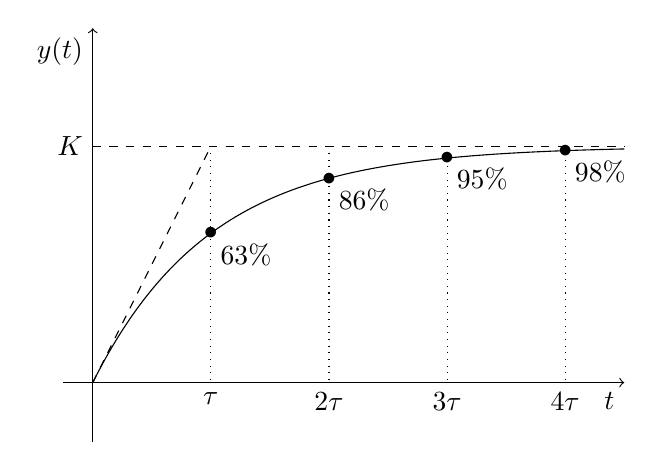
\begin{tikzpicture}[scale=1.5,yscale=2]
	\draw[->] (-0.25,0) -- (4.5,0) node[below left] {$ t $};  % x Axis
	\draw[->] (0,-0.25) -- (0,1.5) node[below left] {$ y(t) $};  % y Axis
	\draw[domain=0:4.5,samples=500] plot (\x,{1-exp(-\x)});
	\draw[dashed] (0,1) node[left] {$ K $}-- (4.5,1);
	\draw[dashed] (0,0) -- (1,1);
	\draw[dotted] (1,1) -- (1,0.63) node{$ \bullet $} node[below right] {$ 63\% $} -- (1,0) node[below] {$ \tau $};
	\draw[dotted] (2,1) -- (2,0.86) node{$ \bullet $} node[below right] {$ 86\% $} -- (2,0) node[below] {$ 2\tau $};
	\draw[dotted] (3,1) -- (3,0.95) node{$ \bullet $} node[below right] {$ 95\% $} -- (3,0) node[below] {$ 3\tau $};
	\draw[dotted] (4,1) -- (4,0.98) node{$ \bullet $} node[below right] {$ 98\% $} -- (4,0) node[below] {$ 4\tau $};
	\end{tikzpicture}
\end{center}
$\tau $ is used as a measure of the system's speed of response. A large time constant means that the system is slow. 1st order systems are characterized by their time constant. This gives you a general idea of how fast the system responds to a step input. Overall, three quantities are used as performance characteristics for 1st-order systems.
\begin{itemize}
	\item Time constant $ \tau $: Time for the step response to rise to 63\% of a final value.
	\item Settling time $ t_s $: Time for a step response to settle to 98\% of the final value.
	\[ t_s=4\tau \]
	\item Rise time $ t_r $: Time taken by step response to go from 10\% to 90\% of the final value.
	\begin{align*}
	y(t) & = K[1-e^{-t/\tau}]1(t)\\
	y(t_1)=0.1\cancel{K} & = \cancel{K}[1-e^{-t_1/\tau}]\\
	e^{-t_1/\tau}& = 1-0.1=0.9\\
	-\frac{t_1}{\tau}& = \ln 0.9 = -0.1054\\
	\Rightarrow\quad t_1 &= 0.1054\tau\\
	y(t_2)=0.9\cancel{K} & = \cancel{K}[1-e^{-t_2/\tau}]\\
	e^{-t_2/\tau}& = 1-0.9=0.1\\
	-\frac{t_2}{\tau}& = \ln 0.1 = -2.3026\\
	\Rightarrow\quad t_2 &=2.3026\tau\\
	t_r &=t_2-t_1 = (2.3026-0.1054)\tau\\
	\Rightarrow\quad t_r &= 2.2\tau
	\end{align*}
	So, rise time for a 1st order system is defined as $ \mathbf{t_r=2.2\tau} $.
\end{itemize}
Note that for 1st-order systems, the slope will always be discontinuous at the origin. So, if you were given the following time-response:
\begin{center}
	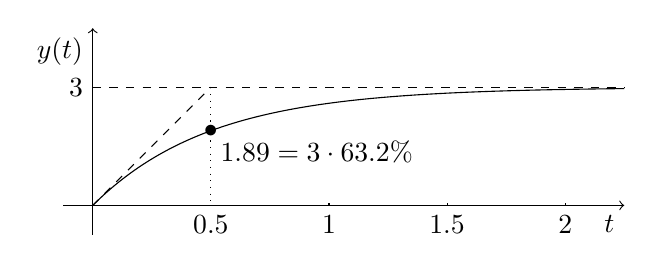
\begin{tikzpicture}[scale=1.5]
	\draw[->] (-0.25,0) -- (4.5,0) node[below left] {$ t $};  % x Axis
	\draw[->] (0,-0.25) -- (0,1.5) node[below left] {$ y(t) $};  % y Axis
	\draw[domain=0:4.5,samples=500] plot (\x,{1-exp(-\x)});
	\draw[dashed] (0,1) node[left] {$ 3 $}-- (4.5,1);
	\draw[dashed] (0,0) -- (1,1);
	\draw[dotted] (1,1) -- (1,0.63) node{$ \bullet $} node[below right] {$ 1.89 = 3\cdot63.2\% $} -- (1,0) node[below] {$ 0.5 $};
	\draw (2,0.02) -- (2,0) node[below] {$1$};
	\draw (3,0.02) -- (3,0) node[below] {$1.5$};
	\draw (4,0.02) -- (4,0) node[below] {$2$};
	\end{tikzpicture}
\end{center}
You should be able to identify the transfer function as
\[ G(s) = \frac{3}{0.5s+1} \]
However if you were given a response like
\begin{center}
	\begin{tikzpicture}[scale=1.5,xscale=1.5]
	\draw[->] (-0.25,0) -- (3,0) node[below left] {$ t $};  % x Axis
	\draw[->] (0,-0.25) -- (0,1.5) node[below left] {$ y(t) $};  % y Axis
	\draw[domain=0:3,samples=500] plot (\x,{1-exp(-(\x)^2)    });
	\draw[dashed] (0,1) -- (3,1);
	\end{tikzpicture}
\end{center}
You know this is not the response of a 1st order system because of its initial slope.

Looking at a pole-zero diagram,
\begin{center}
	\begin{tikzpicture}[scale=1.375]
	\draw (-2.5,0) -- (2.5,0) node[below left] {$ \sigma $};
	\draw (0,-1.5) -- (0,1.5) node[below left] {$ j\omega $};
	\node at (-1.25,0) {\Large$ \times $};
	\node[below] at (-1.25,0) {$ -\frac{1}{\tau}$};
	\end{tikzpicture}
\end{center}
where $ \tau $ is the time constant: the further away the pole is from the $ \jw $-axis, the faster the system response (to a step input).

\section*{2nd Order Systems}
Let's now move to our second case for $ G(s) $: second order systems. A strictly-proper second-order system has a transfer function
\[ G(s)=\frac{b_1s+b_0}{a_2s^2+a_1s+a_0} \]
Let's start by studying 2nd order transfer functions with no zeros.
\[ G(s)=\frac{b_0}{a_2s^2+a_1s+a_0} \]
This is usually written in 1 of 2 ways:
\[ G(s) = \frac{K\gamma_0}{s^2+\gamma_1 s+\gamma_0}\quad or \quad G(s) = \frac{K}{\alpha_2 s^2+\alpha_1 s + 1} \]
In either case, $ K $ is the static gain $ G(0)=K $ assuming both poles of $ G(s) $ are in the LHP. The second-order system has the following response to a step input:
\[ G(s) = \frac{K\gamma_0}{s^2+\gamma_1 s+\gamma_0},\quad U(s) = \frac{1}{s} \]
\[ Y(s)=\frac{K\gamma_0}{s(s^2+\gamma_1 s+\gamma_0)} \]
Initial value:
\[ y(0^+) = \lim_{s\to\infty}sY(s) = 0 \]
Initial slope:
\[ \dot{y}(0^+) = \lim_{s\to\infty}s^2Y(s) = 0 \]
Assuming that the poles of $ G(s) $ are strictly in the LHP, then the final value is:
\[ \lim_{t\to\infty}y(t) = \lim_{s\to0}sY(s) = K \]
So, we have
\begin{center}
	\begin{tikzpicture}[scale=1.5]
	\draw[->] (-0.25,0) -- (4.5,0) node[below left] {$ t $};  % x Axis
	\draw[->] (0,-0.25) -- (0,1.5) node[below left] {$ y(t) $};  % y Axis
	\draw[domain=0:4.5,samples=500] plot (\x,{1-\x*exp(-\x)-exp(-\x)});
	\draw[dashed] (0,1) node[left] {$ K $}-- (4.5,1);
	
	\node at (2.25,-0.625) {or};
	
	\begin{scope}[shift={(0,-2.5cm)}]
	\draw[->] (-0.25,0) -- (4.5,0) node[below left] {$ t $};  % x Axis
	\draw[->] (0,-0.25) -- (0,1.5) node[below left] {$ y(t) $};  % y Axis
	\draw[domain=0:4.5,samples=500] plot (\x,{1-exp(-\x/2)*( sqrt(1/15)*sin( (180/pi)*\x*sqrt(15)/2 ) + cos( (180/pi)*\x*sqrt(15)/2) )});
	\draw[dashed] (0,1) node[left] {$ K $}-- (4.5,1);
	\end{scope}
	\end{tikzpicture}
\end{center}
What happens here depends on the nature of the poles of $ G(s) $.

\paragraph*{Case 1:} $ G(s) $ has 2 real poles.
\[ G(s) = \frac{K\gamma_0}{s^2+\gamma_1 s+\gamma_0} = \frac{K\sigma_1\sigma_2}{(s+\sigma_1)(s+\sigma_2)} \]
(We need the $ \sigma_1\sigma_2 $ term so that $ K $ can continue to be the static gain.) Here, $ \sigma_1 $ and $ \sigma_2 $ are positive real numbers. Let $ \sigma_2>\sigma_1 $.
\begin{center}
	\begin{tikzpicture}[scale=1.375]
	\draw[->] (-2.5,0) -- (2.5,0) node[below left] {$ \sigma $};
	\draw[->] (0,-1.5) -- (0,1.5) node[below left] {$ j\omega $};
	\node at (-1,0) {\Large$ \times $};
	\node[below] at (-1,0) {$ -\sigma_1$};
	\node at (-2,0) {\Large$ \times $};
	\node[below] at (-2,0) {$ -\sigma_2$};
	\end{tikzpicture}
\end{center}
Then the step response is
\[ Y(s) = \frac{K\sigma_1\sigma_2}{s(s+\sigma_1)(s+\sigma_2)} = \frac{R_1}{s}+\frac{R_2}{s+\sigma_1}+\frac{R_3}{s+\sigma_2} \]
\[ R_1 = \left. sY(s)\right|_{s=0} = \frac{K\sigma_1\sigma_2}{\sigma_1\sigma_2}=K \]
\[R_2 = \left. (s+\sigma_1)Y(s)\right|_{s=-\sigma_1} = \frac{K\cancel{\sigma_1}\sigma_2}{(-\cancel{\sigma_1})(-\sigma_1+\sigma_2)} = -\frac{K\sigma_2}{\sigma_2-\sigma_1}\]
\[R_3 = \left. (s+\sigma_2)Y(s)\right|_{s=-\sigma_2} = \frac{K\sigma_1\cancel{\sigma_2}}{(-\cancel{\sigma_2})(-\sigma_2+\sigma_1)} = -\frac{K\sigma_1}{\sigma_1-\sigma_2} = \frac{K\sigma_1}{\sigma_2-\sigma_1}\]
%For brevity, we will define $ \obar{K} = K/(\sigma_2-\sigma_1) $, where $ \obar{K}>0 $. Then,
%\[ R_1=K,\quad R_2 = -\obar{K}\sigma_2,\quad R_3=\obar{K}\sigma_1 \]
So,
\[ Y(s) = \frac{K}{s}-\frac{K\sigma_2}{(\sigma_2-\sigma_1)(s+\sigma_1)}+\frac{K\sigma_1}{(\sigma_2-\sigma_1)(s+\sigma_2)} \]
\[ y(t) = (K-\frac{K\sigma_2}{\sigma_2-\sigma_1}e^{-\sigma_1 t}+\frac{K\sigma_1}{\sigma_2-\sigma_1}e^{-\sigma_2 t})1(t) \]
We see indeed that at $ t=0^+ $:
\[ y(0^+) = K-\frac{K\sigma_2}{\sigma_2-\sigma_1}+\frac{K\sigma_1}{\sigma_2-\sigma_1} = K\left(1-\frac{\sigma_2}{\sigma_2-\sigma_1}+\frac{\sigma_1}{\sigma_2-\sigma_1}\right)=0\]
We can write this as
\[ y(t) = (K - y_{t}(t))1(t)\]
where 
\[ y_{t}(t) = \left(\frac{K}{\sigma_2-\sigma_1}(\sigma_2e^{-\sigma_1t}-\sigma_1e^{-\sigma_2t})\right)1(t) \]
Since $ \sigma_2>\sigma_1 $ (each is positive) and
\[ e^{-\sigma_2t} < e^{-\sigma_1t} \]
\begin{center}
	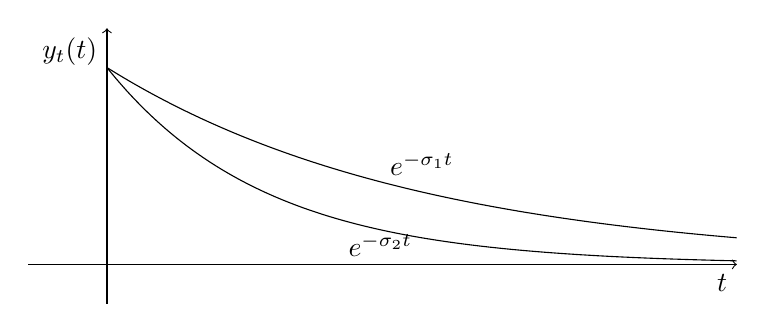
\begin{tikzpicture}[yscale=2,xscale=4]
	\draw[->] (-0.25,0) -- (2,0) node[below left] {$ t $};  % x Axis
	\draw[->] (0,-0.25) -- (0,1.5) node[below left] {$ y_t(t) $};  % y Axis
	\draw[domain=0:2,samples=500] plot (\x,{1.25*exp(-(\x))    });
	\node at (1,0.5) [above] {$ e^{-\sigma_1t} $};
	\draw[domain=0:2,samples=500] plot (\x,{1.25*exp(-2*(\x))    });
	\node at (1,0.25) [below left,align=right] {$ e^{-\sigma_2t} $};
	\end{tikzpicture}
\end{center}
so then
%\[ \sigma_1e^{-\sigma_2t} < \sigma_1e^{-\sigma_1t} \]
\[ \sigma_1e^{-\sigma_2t} < \sigma_2e^{-\sigma_1t} \]
Also given that $ \frac{K}{\sigma_2-\sigma_1}>0 $, then
\[ 0 \leq y_{t}(t) \leq K \]
$ y(t) $ is never greater than $ K $, so no overshoot is possible. This system is said to be \textbf{overdamped}.
\begin{center}
	\begin{tikzpicture}[scale=1.5,yscale=1.5]
	\draw[->] (-0.25,0) -- (4.5,0) node[below left] {$ t $};  % x Axis
	\draw[->] (0,-0.25) -- (0,1.5) node[below left] {$ y(t) $};  % y Axis
	\draw[domain=0:4.5,samples=500] plot (\x,{1-\x*exp(-\x)-exp(-\x)});
	\draw[dashed] (0,1) node[left] {$ K $}-- (4.5,1);
	\end{tikzpicture}
\end{center}
We will now consider a special case of Case 1: $ \sigma_1=\sigma_2=\sigma $ (repeated poles). Then, \[ G(s) = \frac{K\sigma^2}{(s+\sigma)^2} \]
\[ Y(s) = \frac{K\sigma^2}{s(s+\sigma)^2} = \frac{R_1}{s}+\frac{R_2}{(s+\sigma)^2}+\frac{R_3}{s+\sigma}\]
\[ R_1 = K,\quad R_2 = \left.(s+\sigma)^2Y(s)\right|_{s=-\sigma}=\frac{K\sigma^2}{-\sigma} = -K\sigma,\quad R_3 = \frac{d}{ds}\frac{K\sigma^2}{s}\Big|_{s=-\sigma} = \frac{-K\sigma^2}{\sigma^2} = -K \]
\[ Y(s) = \frac{K}{s}-\frac{K\sigma}{(s+\sigma)^2}-\frac{K}{s+\sigma}\]
\[ y(t) = K\left(1-e^{-\sigma t}-\sigma t e^{-\sigma t}\right)1(t) \]
Is $ y(t) $ still bounded by 0 and $ K $, in this case? Let
\begin{itemize}
	\item At $ t=0^+ $: $ e^{-\sigma t} = 1 $, $ \sigma t e^{-\sigma t} = 0 $, $ \Rightarrow\ y(0^+)=0 $.
	\item At $ t\to\infty $: $ e^{-\sigma t} = 0 $, $ \sigma t e^{-\sigma t} \to 0 $, $ \Rightarrow\ \lim\limits_{t\to\infty}y(t)=K $.
	\item Let $ y_{t}(t) =- K\left(e^{-\sigma t}+\sigma t e^{-\sigma t}\right) $ and $ y_{t_2}(t) = \sigma t e^{-\sigma t} $. Our final step is to check the peak location of $ y_{t_2}(t) $. First, find the peak location:
	\[ \dot{y}_{t_2} = \sigma\left(-t\sigma e^{-\sigma t} + e^{-\sigma t} \right) = 0 \]
	\[ e^{-\sigma t} (1-t\sigma) = 0 \quad\Rightarrow\quad t=\frac{1}{\sigma} \]\
	So,
	\[ y_{t_2}\left(\frac{1}{\sigma}\right) = \sigma \frac{1}{\sigma}e^{-\sigma \frac{1}{\sigma}} = e^{-1} \]
	\[ y\left(\frac{1}{\sigma}\right) = K\left(1-e^{-1}-e^{-1}\right)=K-2Ke^{-1} \]
	
	\begin{center}
		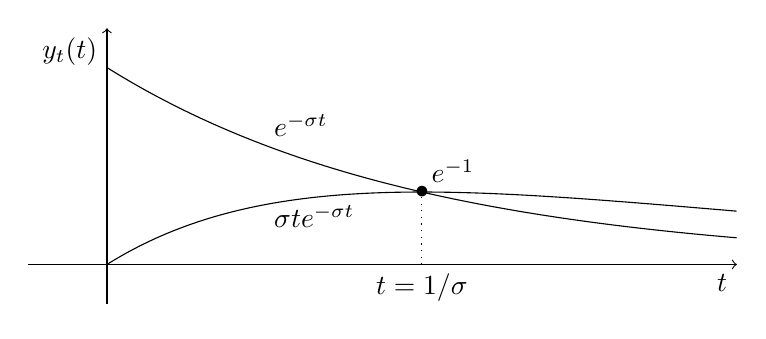
\begin{tikzpicture}[yscale=2,xscale=4]
		\draw[->] (-0.25,0) -- (2,0) node[below left] {$ t $};  % x Axis
		\draw[->] (0,-0.25) -- (0,1.5) node[below left] {$ y_t(t) $};  % y Axis
		\draw[domain=0:2,samples=500] plot (\x,{1.25*exp(-\x)    });
		\node at (0.5,0.75) [above right,align=left] {$ e^{-\sigma t} $};
		\draw[domain=0:2,samples=500] plot (\x,{1.25*\x*exp(-\x)    });
		\draw[dotted] (1,0) node[below] {$ t=1/\sigma $} -- (1,0.46) node {$ \bullet $};
		\node[above right] at (1,0.46) {$ e^{-1} $};
		\node at (0.5,0.4375) [below right,align=left] {$ \sigma te^{-\sigma t} $};
		\end{tikzpicture}
	\end{center}
\end{itemize}
So, $ y(t) $ never exceeds $ K $ nor goes below 0. In fact, repeated poles normally have the fastest 2nd-order response possible without overshoot:
\[ y_{\text{repeated}}(t) > y_{\text{distinct}}(t) \]
%(given that $ \sigma_1 $ is the same for both systems and $ \sigma_2 < \sigma_1 $ for the system with distinct poles).
This system is said to be \textbf{critically damped}. In general, this response looks like a 1st-order response, except that there is no discontinuity in the slope at the origin.

\begin{center}
	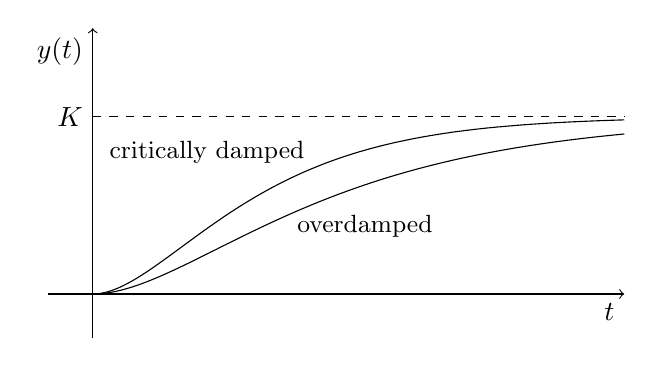
\begin{tikzpicture}[scale=2.25]
	\draw[->] (-0.25,0) -- (3,0) node[below left] {$ t $};  % x Axis
	\draw[->] (0,-0.25) -- (0,1.5) node[below left] {$ y(t) $};  % y Axis
	\draw[domain=0:3,samples=500] plot (\x,{1-2/(2-1)*exp(-\x)+1/(2-1)*exp(-2*\x)});
	\draw[domain=0:3,samples=500] plot (\x,{1-2*\x*exp(-2*\x)-exp(-2*\x)});
	\draw[dashed] (0,1) node[left] {$ K $}-- (3,1);
	\node[left,align=right] at (1.25,0.8) {\small critically damped};
	\node[below right,align=left] at (1.1,0.5) {\small overdamped};
	\end{tikzpicture}
\end{center}

\end{document}

